
% Using KOMA Script document style
% Font size setting and
% option to skip empty lines as new paragraphs
\documentclass[10pt,a4paper]{article}
% Packages without Options
\usepackage{
	algorithm,
	alltt,
	algpseudocode,
	amsfonts,
	amssymb,
	appendix,
	array,
	booktabs,
	dirtree,
	enumitem,
	float,
	footnote,
	gensymb,
	geometry,
	graphicx,
	interval,
	karnaugh-map,
	lipsum,
	listings,
	longtable,
	makecell,
	mathtools,
	minted,
  nicematrix,
	parskip,
	pdfpages,
	pgfkeys,
	pgfplots,
	subcaption,
	tabularx,
	tablefootnote,
	textcomp,
	tikz,
    titlecaps,
	venndiagram,
	wrapfig,
	wrapfig,
	xcolor
}



% Packages with Options

\usepackage[framemethod=tikz]{mdframed}
\usepackage[colorlinks,linkcolor=cyan, citecolor=cyan, urlcolor=cyan]{hyperref}
\usepackage[labelfont=bf,textfont=it,labelsep=period]{caption}
\usepackage[RPvoltages]{circuitikz}
\usepackage[english]{babel}
\usepackage[nameinlink,noabbrev]{cleveref}

\definecolor{mintedbackground}{rgb}{0.97,0.97,0.97}

\setminted[cpp]{
bgcolor=mintedbackground,
    linenos=true,
    breaklines=true,}

\setminted[js]{
bgcolor=mintedbackground,
    linenos=true,
    breaklines=true,}

\setminted[python]{
bgcolor=mintedbackground,
    linenos=true,
    breaklines=true,}
    

\linespread{1.5}

% Package: AlgorithmicX
% Sets all comments to be indentend and aligned

\renewcommand{\Comment}[2][.7\linewidth]{%
  \leavevmode\hfill\makebox[#1][l]{//~#2}}


% Package: Interval
% Sets the style of mathematical intervals
\intervalconfig{
soft open fences, separator symbol=,,
}

% Package: Geometry
% Sets the page margins
\geometry{
    a4paper,
    left=32mm,
    right=22mm,
    top=22mm,
    }
	
% Creates a proper caption name for algorithms
\newcommand{\algorithmautorefname}{Algorithm}
\newcommand{\listingautorefname}{Listing}
\algrenewcommand{\algorithmiccomment}[1]{\texttt{// #1} }
% Creates a numbered environment for Theorems
\newtheorem{theorem}{Theorem}

% Redefine the implication arrow to be a simple, thin arrow instead of the default, thick arrow
\renewcommand{\implies}{\rightarrow}

% Create a new command for the set complement to make my logical statements easier to read
\newcommand{\compl}{\overline}

% Creates commands for combinatorics nCr and nPr
\newcommand{\nCr}[2]{\,_{#1}C_{#2}} % nCr
\newcommand{\nPr}[2]{\,_{#1}P_{#2}} % nPr

% Package: tikz
% Loads libraries for drawing automata, 
\usetikzlibrary{automata,positioning,shadows,arrows, shapes.gates.logic.US, calc}

% Creates a command to create a button shape
\newcommand*\keystroke[1]{%
  \tikz[baseline= (key.base)]
    \node[%
      draw,
      fill=white,
      drop shadow={shadow xshift=0.25ex,shadow yshift=-0.25ex,fill=black,opacity=0.75},
      rectangle,
      rounded corners=2pt,
      inner sep=1pt,
      line width=0.5pt,
      font=\scriptsize\sffamily
    ] (key) {#1\strut};
}

% Package: pgfplot
% Sets the global options for PGF Plots
\pgfplotsset{compat=newest}

% Package: tikz
% Flowchart Shapes
\tikzstyle{startstop} = [rectangle, rounded corners, minimum width=3cm, minimum height=1cm,text centered, draw=black, fill=red!30]
\tikzstyle{io} = [trapezium, trapezium left angle=70, trapezium right angle=110, minimum width=3cm, minimum height=1cm, text centered, draw=black, fill=blue!30]
\tikzstyle{process} = [rectangle, minimum width=3cm, minimum height=1cm, text centered, draw=black, fill=orange!30]
\tikzstyle{decision} = [diamond, minimum width=3cm, minimum height=1cm, text centered, draw=black, fill=green!30]
\tikzstyle{arrow} = [thick,->,>=stealth]

% Disable Minted syntax error highlights (red boxes)
\AtBeginEnvironment{minted}{%
  \renewcommand{\fcolorbox}[4][]{#4}}

% Listings Style (non-minted)

\lstdefinestyle{arjuncode}{
    basicstyle=\ttfamily,
    breakatwhitespace=false,         
    breaklines=true,                 
    captionpos=b,                    
    keepspaces=true,                 
    numbers=left,                    
    numbersep=5pt,                  
    showspaces=false,                
    showstringspaces=false,
    showtabs=false,                  
    tabsize=2
}

\lstset{style=arjuncode}

\graphicspath{{images/}}

 %Adjust this based on where your Summary is stored
\title{CM2040: Databases, Networks and the Web \\ Summary}
\author{Arjun Muralidharan}
\begin{document}

\maketitle
\newpage
\tableofcontents
\listoffigures
\listoftables
% \listofalgorithms

\newpage
\renewcommand{\subsubsectionautorefname}{section\negthinspace}

\section{Three-tier web applications}
\begin{mdframed}

\paragraph{Key Concepts}
\begin{itemize}[label={\checkmark}]
\item Intro to module and lab
\item Static vs. dynamic web applications
\item 3-tier web applications architecture
\end{itemize}

\paragraph{Learning Outcomes}
\begin{itemize}[label={\checkmark}]
\item Recognize the tools available for this module to edit a Node file and run it
\item Describe what static and dynamic web applications are
\item Describe what a 3-tier web application architecture is
\end{itemize}
\end{mdframed}
\subsection{Static vs. Dynamic Web Applications}
A \textbf{web application} is a client-server software application in which the user interface runs in a web browser. It could be a computer program which allows a user to submit and retrieve data to or from a database over the Internet using their preferred browser. It is an application in which all or some parts of the software are downloaded from the web each time it is run.

\textbf{Static web applications} are static internet resources with little to no interaction with the user. \textbf{Dynamic web applications} have more user interactions, and users can input, change and manipulate data. 

Differences between web applications and desktop applications are shown in \autoref{tab:desktopvsweb}.

\begin{table}[ht]
    \centering
    \begin{tabular}{@{}ll@{}}
    \toprule
    \textbf{Desktop} & \textbf{Web} \\ \midrule
    Accessed through OS & Accessed through browser \\
    Different appearance/experience in each OS & Consistent appearance/experience across platforms \\
    Access to system resources; fast & Less access to system resources; slow \\
    Lower risk of data loss & Higher risk of data loss \\
    Different version for each OS & Same version across all platforms \\
    Multiple updates required & Single update for all users \\ \bottomrule
    \end{tabular}
    \caption{Desktop vs.\ Web Applications}
    \label{tab:desktopvsweb}
    \end{table}

    \subsubsection{Lifetime of a web request}
When a (static) web application is accessed, the following steps occur in order.

\begin{enumerate}
    \item A \textbf{URL} is typed into the browser
    \item Browser cache is checked; if the application is already available, the procedure skips to the last step
    \item \textbf{DNS} lookup finds the \textbf{IP} address of the server
    \item Browser initiates a \textbf{TCP} connection with the server
    \item Browser sends an \textbf{HTTP} request to the server
    \item Server handles the incoming request 
    \item Browser receives the \textbf{HTTP} response
    \item Browser displays the \textbf{HTML} content 
\end{enumerate}

\subsubsection{Accessing remote resources with HTTP}
\textbf{HTTP} is a \emph{client-server application protocol}. The client sends a request and a server provides a response.

\textbf{HTTP requests}  have a fixed format, which consists of three parts: a \textbf{request line} , some optional message \textbf{headers} , and the \textbf{request body}  (also optional).
The request line is a formatted string, which consists of three parts; the HTTP method (e.g.\ \texttt{GET} or \texttt{POST}), the URL of the requested resource, and the protocol version. For example, the following request line: 
\begin{minted}{http}
    GET /unbound/flashbks/computer/bushf.htm HTTP/1.1
\end{minted}

A server responds with an HTTP response message, which is structured in three parts: a \textbf{status line} , a set of optional \textbf{headers} , and a \textbf{message body}.

The status line consists of the protocol version followed by a numeric status code and its associated message, e.g.

\begin{minted}{http}
    HTTP/1.1 404 Not found
\end{minted}

HTTP is \textbf{stateless}. Each call is treated independently and there is no information maintained between two successive requests. HTTP cannot maintain a user session.

HTTP is \textbf{pull-based}. Only the client can initiate a request-response action, the server cannot contact the client.

\paragraph{Header Types }There are four kinds of \textbf{headers}:
\begin{enumerate}
    \item \textbf{General headers}: These apply to both the request and response, e.g.\ Date
    \item \textbf{Request headers}: Specific to requests, e.g.\ Accept-Language, which sends which response languages are acceptable
    \item \textbf{Response headers}: Specific to responses, e.g. WWW-Authenticate which returns if a user is authorized or not
    \item \textbf{Entity headers}: Apply to the content of the request or response body, e.g.\ Content-Length specifies the length (in bytes) of the body
\end{enumerate}

However, these notions are valid as of HTTP1.1 and may not be valid in HTTP/2 and newer versions.

\subsection{Three-tier application architecture}
The core principle of \textbf{three-tier architectures}  is to provide an intermediate layer between the client and the data tier, which centralizes middleware services and the business logic of the application. Three-tier architectures offer a higher degree of scalability than two-tier con- figurations, thanks to better network utilization and to the virtually unlimited replication and load distribution capabilities of the middle tier. A comparison is shown in \autoref{threetier}.

\begin{figure}[ht]
    \centering
    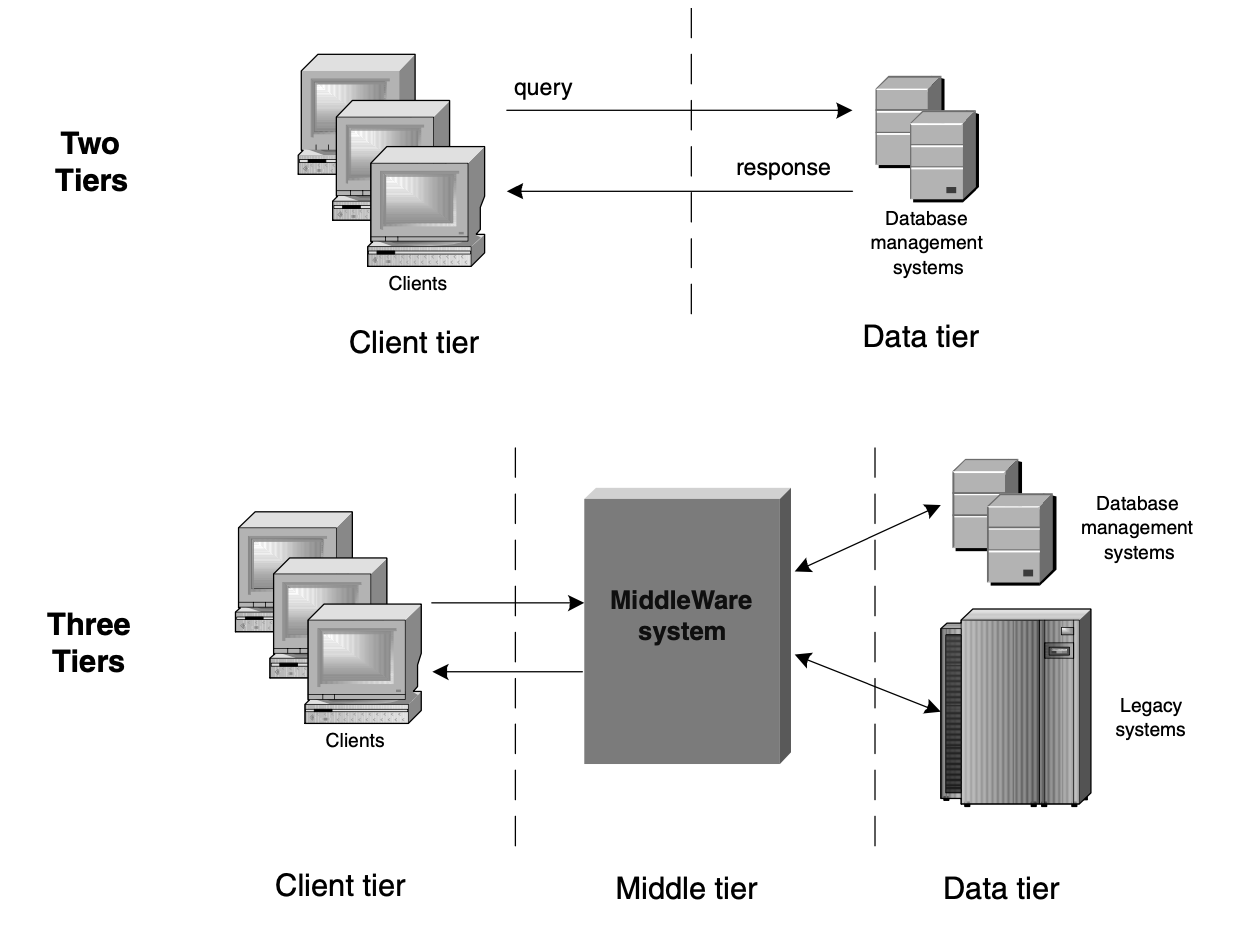
\includegraphics[width=\textwidth]{threetier.png}
    \caption{Two-tier vs.\ three-tier architecture}
    \label{threetier}
\end{figure}


\section{Building simple web servers}

\begin{mdframed}

\paragraph{Key Concepts}
\begin{itemize}[label={\checkmark}]
\item Web server and web hosting
\item How to build a simple web server with Node
\item Building an Express web server
\end{itemize}

\paragraph{Learning Outcomes}
\begin{itemize}[label={\checkmark}]
\item Explain what a web server is
\item How to build a simple web server with Node.js
\item Building an Express web server

\end{itemize}
\end{mdframed}
\subsection{Web servers}
A \textbf{web server} is a program that uses HTTP to serve the files that form web pages to users, in response to their requests, which are forwarded by their computers' HTTP clients.

A basic web server architecture includes:

\begin{itemize}
	\item Hardware
	\item Operating system
	\item HTTP server
	\item Database \emph{(optional)} 
	\item Scripting Language \emph{(optional)} 
\end{itemize}

The \textbf{HTTP server} compiles the results from databases and scripting language, and controls what options are available to the end user via \textbf{configuration files} . 

\subsection{Node.js}
\textbf{Node.js} is an asynchronous, event-driven Javascript runtime environment. It is not a programming language or development framework.

In an \textbf{asynchronous} environment, events can happen at different times, i.e. the timing of events doesn't matter. Node.js responds to any request immediately, as opposed to synchronous environments such as PHP, that handles one request at a time, and subsequent requests wait. The differences are shown in \autoref{tab:nodevsphp}.


\begin{table}[ht]
    \centering
    \begin{tabular}{@{}ll@{}}
    \toprule
    \textbf{Node.js} & \textbf{PHP} \\ \midrule
    Asynchronous & Synchronous \\
    Single-threaded & Multi-threaded \\
    Non-blocking & Blocking \\
    Highly scalable & Less scalable \\
    Memory-efficient & Less memory-efficient \\
    Able to share code between browser and server & --- \\ \bottomrule
    \end{tabular}
    \caption{Node.js vs.\ PHP}
    \label{tab:nodevsphp}
    \end{table}

Node.js is suitable for \textbf{I/O-intensive applications} such as social media websites, but not suitable for \textbf{CPU-intensive applications} such as CAD software or games. 



\section{Generating web pages from data using templates}

\begin{mdframed}

\paragraph{Key Concepts}
\begin{itemize}[label={\checkmark}]
\item Routing in dynamic web applications
\item Separation of Concern (SoC)
\item Rendering html files and Templating
\end{itemize}

\paragraph{Learning Outcomes}
\begin{itemize}[label={\checkmark}]
\item Describe and apply routing in web server development
\item Describe and apply Separation of Concern principle of programming in your web application development
\item Describe and apply templating in web application
\end{itemize}


\end{mdframed}

\subsection{Routes}
\textbf{Routes}  are URL schema, which describe the interfaces for making requests to your web app. Combining an HTTP request method (a.k.a. \texttt{HTTP verb}) and a path pattern, you define URLs in your app.

Each route has an associated route handler, which does the job of performing any action in the app and sending the HTTP response.

\begin{minted}{js}
	app.get("/about", (req, res) => res.send("<h1>This is the about page</h1>")); 
\end{minted}

\begin{figure}[H]
	\centering
	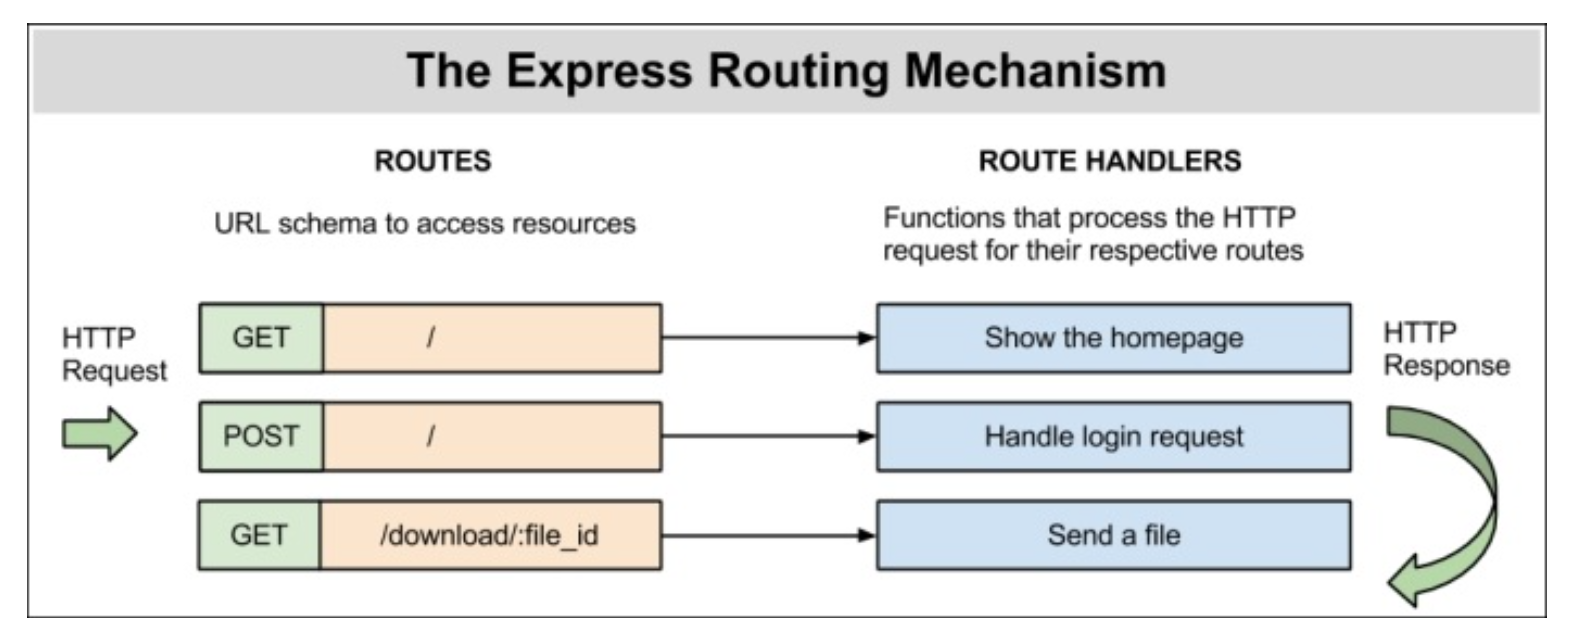
\includegraphics[width=\textwidth]{routing.png}
	\caption{Express Routing Mechanism}
	\label{fig:routing}
\end{figure}
\subsection{Separation of Concerns}
\textbf{Separation of Concerns} is a \emph{design principle} for an application such that each module or layer in an application should only be responsible for one thing and should not contain code that deals with other things.

SoC is achieved by 
\begin{enumerate}
	\item constructing a modular application through encapsulation
	\item layering functionality in the application, e.g. such as a three-tier architecture which is loosely coupled
\end{enumerate}

The objective is to remove as many dependencies as possible between the individual parts.

Benefits of SoC include:

\begin{enumerate}
	\item Reduces complexity
	\item Helps \textbf{DRY} (``Don't repeat yourself'') 
	\item Improves portability
	\item Improves maintainability and testability
\end{enumerate}

\subsection{Templating}
A \textbf{template engine} can help produce a dynamic HTML page by \textbf{inserting variables} into the final output, and \textbf{running programming logic} at run-time before sending the final HTML output to the browser.

This helps keep the logic in the HTML file at a minimum. Popular template engines include \textbf{EJS}, \textbf{Pug} and \textbf{Mustache}.

\textbf{EJS} template files use HTML and EJS tags:
\begin{lstlisting}
	<%= %> 
\end{lstlisting}
used to output the return value of an expression into the document.
\begin{lstlisting}
	<% %> 
\end{lstlisting}
used to evaluate an expression, but not add the return value to the document.
An example:
\begin{minted}{html}
 <h1><%=title%></h1>
 <ul>
	<%for (var i=0; i < supplies.length; i++) {%>
		<li>
			<a href="supplies/<%=supplies[i]%>"></a>
		</li>
	<%}%>
</ul>
\end{minted}
The parameters, such as \texttt{title}, can be set in a JavaScript file that define the routes. These are usually located in the \emph{main.js} file in \emph{routes}.  


\section{Handling forms to input data}

\begin{mdframed}

\paragraph{Key Concepts}
\begin{itemize}[label={\checkmark}]
    \item Form handling and HTTP GET and POST methods
    \item HTTP GET method, form handling and collecting form-data
    \item HTTP POST method, form handling and collecting form-data
\end{itemize}

\paragraph{Learning Outcomes}
\begin{itemize}[label={\checkmark}]
\item Describe and apply form handling in their web application
\item Describe and apply GET and POST request methods in dynamic web application
\item Describe and run the code to retrieve form data in middleware
\end{itemize}
\end{mdframed}

\subsection{GET and POST methods}
The \texttt{GET} HTTP method is used to request a resource on a server, while \texttt{POST} sends data to a resource on the server.

\texttt{GET} may never manipulate any data. \texttt{POST} is commonly used with web forms to send data to a server or to retrieve sensitive data (by providing credentials).

\subsection{GET}

Routes for an HTTP \texttt{GET} method can be invoked with the following Express command. The method requests the resources from the server but can also pass form input fields via the URL. This is useful for simple data that doesn't need to be stored and is not sensitive.
\begin{minted}{js}
	app.get("/search-result", function (req, res) {
		//searching in the database
		res.send(
			"This is the keyword you entered: " +
				req.query.keyword +
				"<br />" +
				"This is the result of the search:"
		);
	});
   \end{minted}

\section{Representing data in databases, relational databases}

\begin{mdframed}

\paragraph{Key Concepts}
\begin{itemize}[label={\checkmark}]
\item Introduction to databases
\item Relational databases
\item MySQL shell
\end{itemize}

\paragraph{Learning Outcomes}
\begin{itemize}[label={\checkmark}]
\item Describe what a list of data is
\item Describe modification problems related to lists of data
\item Describe what a relational database is 
\end{itemize}
\end{mdframed}

\subsection{Relational Databases}
The \textbf{database approach} to managing and accessing data has \textbf{key characteristics}:

\paragraph{Self-describing nature} A database system contains a complete definition of the database structure and constraints, stored in the \textbf{DBMS catalog} and called \textbf{meta data}. NOSQL systems are designed to not requires a catalog.

\paragraph{Insulation between programs and data, and data abstraction} With a DBMS, the structure of the data can be extended or even changed \textbf{without programs having to change}  (e.g., adding a new attribute). Some databases provide an \textbf{object-oriented system} , allowing to define an interface describing the data names and types, and the implementation contains the actual operation, which can change without breaking the interface.

\paragraph{Support for multiple views of the data} Data can be served in subsets tailored for specific users, and data can be \textbf{virtual data}, which is derived from the stored data but not actually stored (e.g. a calculated field).

\paragraph{Sharing of data and multiuser transaction processing} A DBMS includes \textbf{concurrency control} software, ensuring multiple users can interact with the data at the same time. A \emph{transaction} is a process with one or multiple database accesses. The \textbf{isolation} property ensures that a transaction appears to execute in isolation from other transactions. \textbf{Atomicity} ensures that either all database operations in a transaction are executed, or none are.

The DBMS approach further reduced \textbf{redundancy} by \textbf{normalizing data}, i.e. storing a logical data item in only a single place.


\subsection{MySQL Shell}
The MySQL shell can be accessed and quit with 
\begin{minted}{shell}
	# Invoke the mysql shell with with user root and ask for password 
	mysql -u root -p
	
	# Exit the mysql shell
	exit
\end{minted}
with the following basic SQL commands available.

\begin{minted}{sql}
	--Create a database names "myRestaurantMenu"
	CREATE DATABASE myRestaurantMenu;

	--Show all databases on the system
	SHOW DATABASES;
	
	--Switch to a specific database named "myBookShop"
	USE myBookShop;

	--Show the available tables
	SHOW TABLES;


\end{minted}

\subsection{Creating Tables}
SQL tables are created using the \texttt{CREATE TABLE} command specifying the data types and constraints for each field. The most common constraints to use are \texttt{NOT NULL} to specify that an attribute may not be \texttt{NULL},  \texttt{DEFAULT} \( i \)  to specify a default value of \( i \) and \texttt{AUTO\_INCREMENT} to specify integer values that automatically increment as rows are added.

\begin{minted}{sql}
CREATE TABLE dishes
(
id INT AUTO_INCREMENT,
name VARCHAR(50),
price DECIMAL(5, 2) unsigned,
is_vegetarian BOOLEAN,
is_vegan BOOLEAN,
PRIMARY KEY(id)
);
\end{minted}

\subsection{Inserting data}

Inserting data is done using the \texttt{INSERT} command and specifying values with the \texttt{VALUES} keyword.

\begin{minted}{sql}
INSERT INTO
	dishes (name, price, is_vegetarian, is_vegan)
VALUES
	('pizza margherita', 10.99, 1, 0),
	('soya burger', 9.50, 1, 1);
\end{minted}


\subsection{Querying data}
Basic SQL queries follow the \texttt{SELECT-FROM-WHERE} structure.

\begin{minted}{sql}
SELECT name, price
FROM dishes
WHERE price > 1;

--Using wildcards and limits
SELECT *
FROM dishes
LIMIT 2;
\end{minted}

This structure is also used to perform deletion und updates of data.

\begin{minted}{sql}
--Delete rows
DELETE FROM
	dishes
WHERE
	price > 1;

--Update rows
UPDATE
	dishes
SET
	price = 2
WHERE
	price = 1;	
\end{minted}

\section{Basic database operations, providing access to databases from middleware}

\begin{mdframed}

\paragraph{Key Concepts}
\begin{itemize}[label={\checkmark}]
\item Basic SQL, review create, select and insert into and introduce update and delete
\item Primary keys
\item Access to database from middleware

\end{itemize}

\paragraph{Learning Outcomes}
\begin{itemize}[label={\checkmark}]
\item Describe and apply statements in SQL to do basic database operations. 
\item Describe and apply primary key and foreign keys in relational databases
\item Recognize and apply access to databases from middleware code in Node to build dynamic web applications

\end{itemize}
\end{mdframed}

\subsection{Primary Keys}
A primary key is a field or combination of fields in a table that \textbf{uniquely} identifies each row or record. It is declared when creating a table using the \texttt{PRIMARY KEY} directive.

Mostly, a primary key is a \textbf{numerical} field and is set to automatically increment (\texttt{AUTO\_INCREMENT}).

\subsubsection{Integrity Constraints}
Table fields can be defined with constraints such as \texttt{UNIQUE}, \texttt{NOT NULL} and  \texttt{DEFAULT} to support the structural integrity of the database. Primary keys have some built-in constraints:
\begin{itemize}
	\item Every table must have a primary key field or combination of fields.
	\item This is equivalent to \texttt{UNIQUE} and \texttt{NOT NULL} constraints.
\end{itemize}

\subsection{Passing variables to the back end}
Data from an application can be passed to the back end and stored in the database by constructing an SQL query in code and using the appropriate function to invoke that query with the variable passed in. In Express, placeholder question marks ()\texttt{?}) are used in the SQL statement, which can then be filled up by a variable. This variable can be a single value or an array of values.

\begin{minted}{js}
app.post("/bookadded", function (req,res) {

// saving data in database
let sqlquery = "INSERT INTO books (name, price) VALUES (?,?)";

// execute sql query
let newrecord = [req.body.name, req.body.price];
db.query(sqlquery, newrecord, (err, result) => {
	if (err) {
		return console.error(err.message);
		}
	else res.send(" This book is added to database, name: "
					+ req.body.name 
					+ " price "
					+ req.body.price);
		});
});
\end{minted}

The input to the query can be sanitized using a sanitizer to clean up data and prevent malicious code injection.

\section{Building a dynamic web application}

\begin{mdframed}
\paragraph{Key Concepts}
\begin{itemize}[label={\checkmark}]
\item Passing variables from middleware to front- end (templates)
\item Passing variables from middleware to backend (database)
\item Review what you have learned so far for development of a dynamic web application
\end{itemize}

\paragraph{Learning Outcomes}
\begin{itemize}[label={\checkmark}]
\item Create a complete dynamic web application performing basic database operations
\item Describe and apply passing variables from middleware to front-end (templates)
\item Describe and apply passing variables from middleware to backend (database)
\end{itemize}
\end{mdframed}

The web applications built with Express, Node and SQL Server are an example of \textbf{event-driven programming} as opposed to sequential programming.  The flow of the program is determined based on events, such as user inputs or sensor outputs.

\section{Database schema, ERD}



\begin{mdframed}

\paragraph{Key Concepts}
\begin{itemize}[label={\checkmark}]
\item Database schema
\item Junction (bridge) tables
\item SQL Join
\end{itemize}

\paragraph{Learning Outcomes}
\begin{itemize}[label={\checkmark}]
\item Explain the context behind the relational model and describe the process of schema development
\item Explain the context behind the junction (bridge) tables in relational model and describe the process of schema development
\item Explain and apply foreign keys in relational databases
\item Perform queries on databases using multiple related tables by JOIN queries
\end{itemize}
\end{mdframed}




\subsection{Database schema}

To develop a \textbf{conceptual schema} of a database, we first identify the \textbf{entities}, \textbf{attributes}, and \textbf{data types} in the database.

Next, decide the \textbf{primary key} for each entity, \textbf{relationships} between entities and the respective \textbf{foreign keys} and, finally, identify the \textbf{relationship cardinalities} to proceed to refining the databse design.  

Entity relationship diagrams are denoted using the notation shown in \autoref{notation}.

\begin{figure}[H]
	\centering
	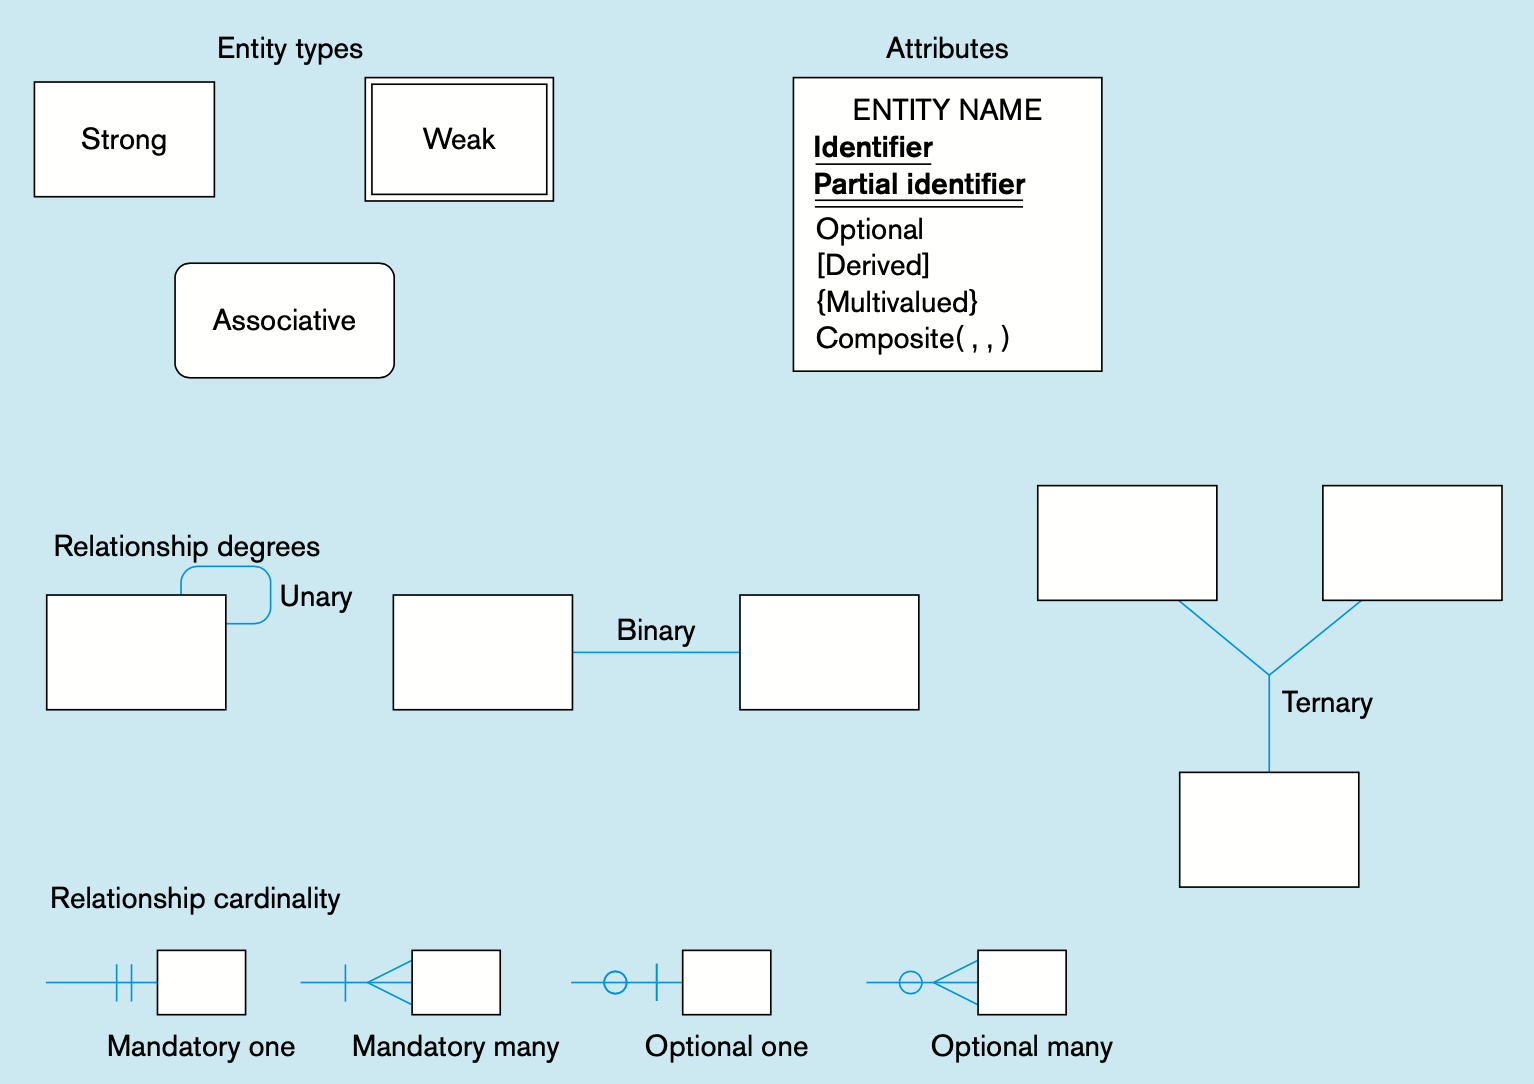
\includegraphics[width=\textwidth]{notation.png}
	\caption{ER Diagram Notation}
	\label{notation}
\end{figure}

Alternative notations use the concept of \textbf{total relationships}, denoting that an entity's existence depends on the presence of one or more relationships, or \textbf{partial relationships}, stating that entities can exist with or without the relationship. These denoted with single or double lines between the entity and the relationship.  

\subsection{Foreign Keys and SQL Join}
A \textbf{foreign key} is an attribute of an entity that is also the \emph{primary key} of another entity that is related to the original entity.

Foreign keys are declared with the respective constraint and ensure the referential integrity of the data by \textbf{limiting the content of the foreign key}  to the values of the referenced primary key.

To combine attributes from two tables, we can use a \texttt{JOIN} statement.

\begin{minted}{sql}
	SELECT * FROM table1
	JOIN table2
	ON table1.attribute = table2.attribute
	WHERE table1.anotherAttribute = criterion;
\end{minted}

In the example above, the attribute from table 1 is the foreign key, while the attribute from table 2 is usually the primary key, but not restricted to it.

\section{Querying a database (advanced)}

\begin{mdframed}

\paragraph{Key Concepts}
\begin{itemize}[label={\checkmark}]
\item Aggregate functions in SQL
\item Left and right joins in SQL
\item Nested select in SQL
\end{itemize}

\paragraph{Learning Outcomes}
\begin{itemize}[label={\checkmark}]
\item Perform advanced queries on databases using aggregate functions
\item Perform advanced queries on databases using multiple related tables by LEFT and RIGHT JOIN queries
\item Perform advanced queries on databases using multiple related tables by nested SELECT queries
\end{itemize}
\end{mdframed}

\subsection{Aggregate Functions}
Aggregate functions allow summarizing tuples of data into a single-tuple summary. In other words, aggregate functions query a database and summarize the data into a single row.

Common aggregate functions are \texttt{SUM}, \texttt{COUNT}, \texttt{MIN}, \texttt{MAX} and \texttt{AVG}, and they do exactly what one would expect them to do.

\subsection{LEFT and RIGHT JOIN}
A normal \texttt{JOIN} statement returns only records at the intersection \( A \cap B\) of two tables \( A \) and \( B \). This is also sometimes called \texttt{INNER JOIN}.

A \texttt{LEFT JOIN} returns all the records from \( A \), completed with matching attributes from \( B \). A \texttt{RIGHT JOIN} does the opposite.  

\subsection{Nested SQL Queries}

The argument to a \texttt{WHERE} clause can itself be an SQL subquery returning a value for comparison.

\begin{minted}{sql}
	SELECT name, price FROM food WHERE price=(SELECT MAX(price) FROM food)
\end{minted}

\section{Networking concepts}

\begin{mdframed}

\paragraph{Key Concepts}
\begin{itemize}[label={\checkmark}]
\item Basic concepts of computer networking
\item TCP/IP model and network protocol
\end{itemize}

\paragraph{Learning Outcomes}
\begin{itemize}[label={\checkmark}]
\item Explain and apply the basic concepts of computer networking
\item Describe TCP/IP model and layers in the model 
\item Identify network protocols in each layer
\end{itemize}
\end{mdframed}

\subsection{Packet switching}
In \textbf{packet switching} , unlike in circuit switching, each data unit to be transferred by the network doesn't know the entire path to the destination. It only knows the destination address.

Intermediate devices in the network locally decide the path and forward to the next known node that is closer to the destination.

\subsection{The TCP/IP model}
The \textbf{Transmission Control Protocol (TCP)/Internet Protocol (IP)} , which is an Internet protocol stack to perform communications between two computers, or hosts, through the Internet. It is a collection of different protocols. A \emph{protocol}  is a set of rules that controls the way data is trans- mitted between hosts.

The open systems interconnection reference model provides an abstraction of networking, as shown in \autoref{osimodel}.

\subsubsection{Application Layer}
The \textbf{application layer} is the highest layer in the OSI stack and closest to the user. Example protocols are HTTP, FTP, SMTP, SSH, DNS, DHCP and Telnet.

This layer defines the type of messages exchanged, such as request/response, defines the fields in the messages and the meaning of fields.

SSL (older) and TLS (newer) are additional layers used to encrypt data at the application layer.

\subsubsection{Transport Layer}
The main protocol at the \textbf{transport layer} is \textbf{TCP}, which handles establishing of connections, checking their reliability, error checking and a three-way handshake process:
\begin{enumerate}
	\item Client host sends \texttt{TCP SYN} segment to server.
	\item Server host receives \texttt{SYN}, replies with \texttt{SYNACK}.
	\item Client receives \texttt{SYNACK}, replies with \texttt{ACK}, which may also contain data.
\end{enumerate}

An alternative to TCP is UDP, or \textbf{user datagram protocol} which does not provide error-checking or handshaking, making it suitable for high-speed applications such as live broadcasting, gaming or video conferencing. TCP is more suited to transfering documents and data reliably.

In addition to an \textbf{IP address}, a \textbf{port} defines which application receives specific data.

\textbf{Multiplexing} allows collecting multiple data segments from various ports and sending them out. \textbf{De-multiplexing} does the opposite, checking each received datagram and delivering it to the correct port.  


\subsubsection{Network Layer}
The main protocol at the network layer is the \textbf{Internet Protocol} or \textbf{IP}. IPv4 addresses are 32-bit numbers, divided into four 8-bit sections ranging from 0 to 255.

IPv6 addresses are 128-bit numbers divided into eight 16-bit sections, each represented by 2 hexadecimal octets.

\textbf{Routing} is a mechanism carrying packers from source to destination, using the IP address, by a hop-by-hop process.

To prevent packets from being passed on infinitely, a TTL (time to live) value is initialised in the packet, and each time the packet is forwarded, the value is reduced by 1. When it reaches 0, the packet has lived too long and gets destroyed.

\subsubsection{Link Layer}
The link layer gets data across one hop, using protocols based on the medium at the physical layer, such as wire, Wi-Fi, fibre-optic and ethernet.

\textbf{Frames} use hardware-specific addressing such as media access control \textbf{MAC addresses}.

\begin{figure}[H]
	\centering
	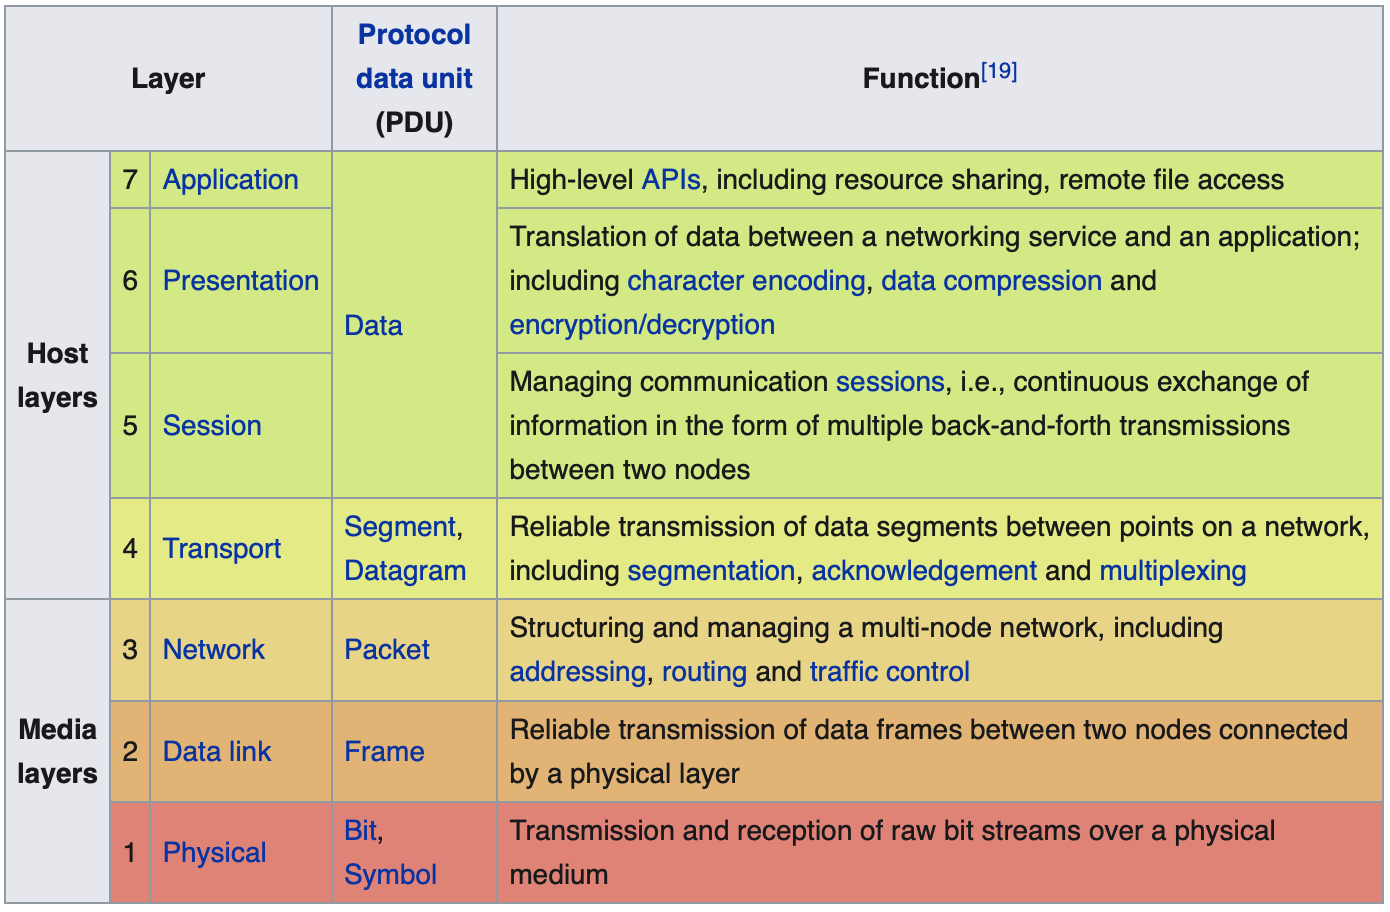
\includegraphics[width=\textwidth]{osi}
	\caption{OSI reference model}
	\label{osimodel}
\end{figure}

\end{document}

